
\chapter{Data analysis}

In this chapter our data sample will be analyzed according to the framework provided by Yoshikata Hatta. The angular correlation of jets is taken, and event mixing is used to factor out acceptance effects. 

[Something about the MC generation \cite{lheFormat}]

The $\phi$ distribution was taken for the data and gen-level MC. Figure \ref{fig:rawPhi} shows the $\phi$ distribution before the application of any corrections. 

\begin{figure}[h!]
\begin{centering}
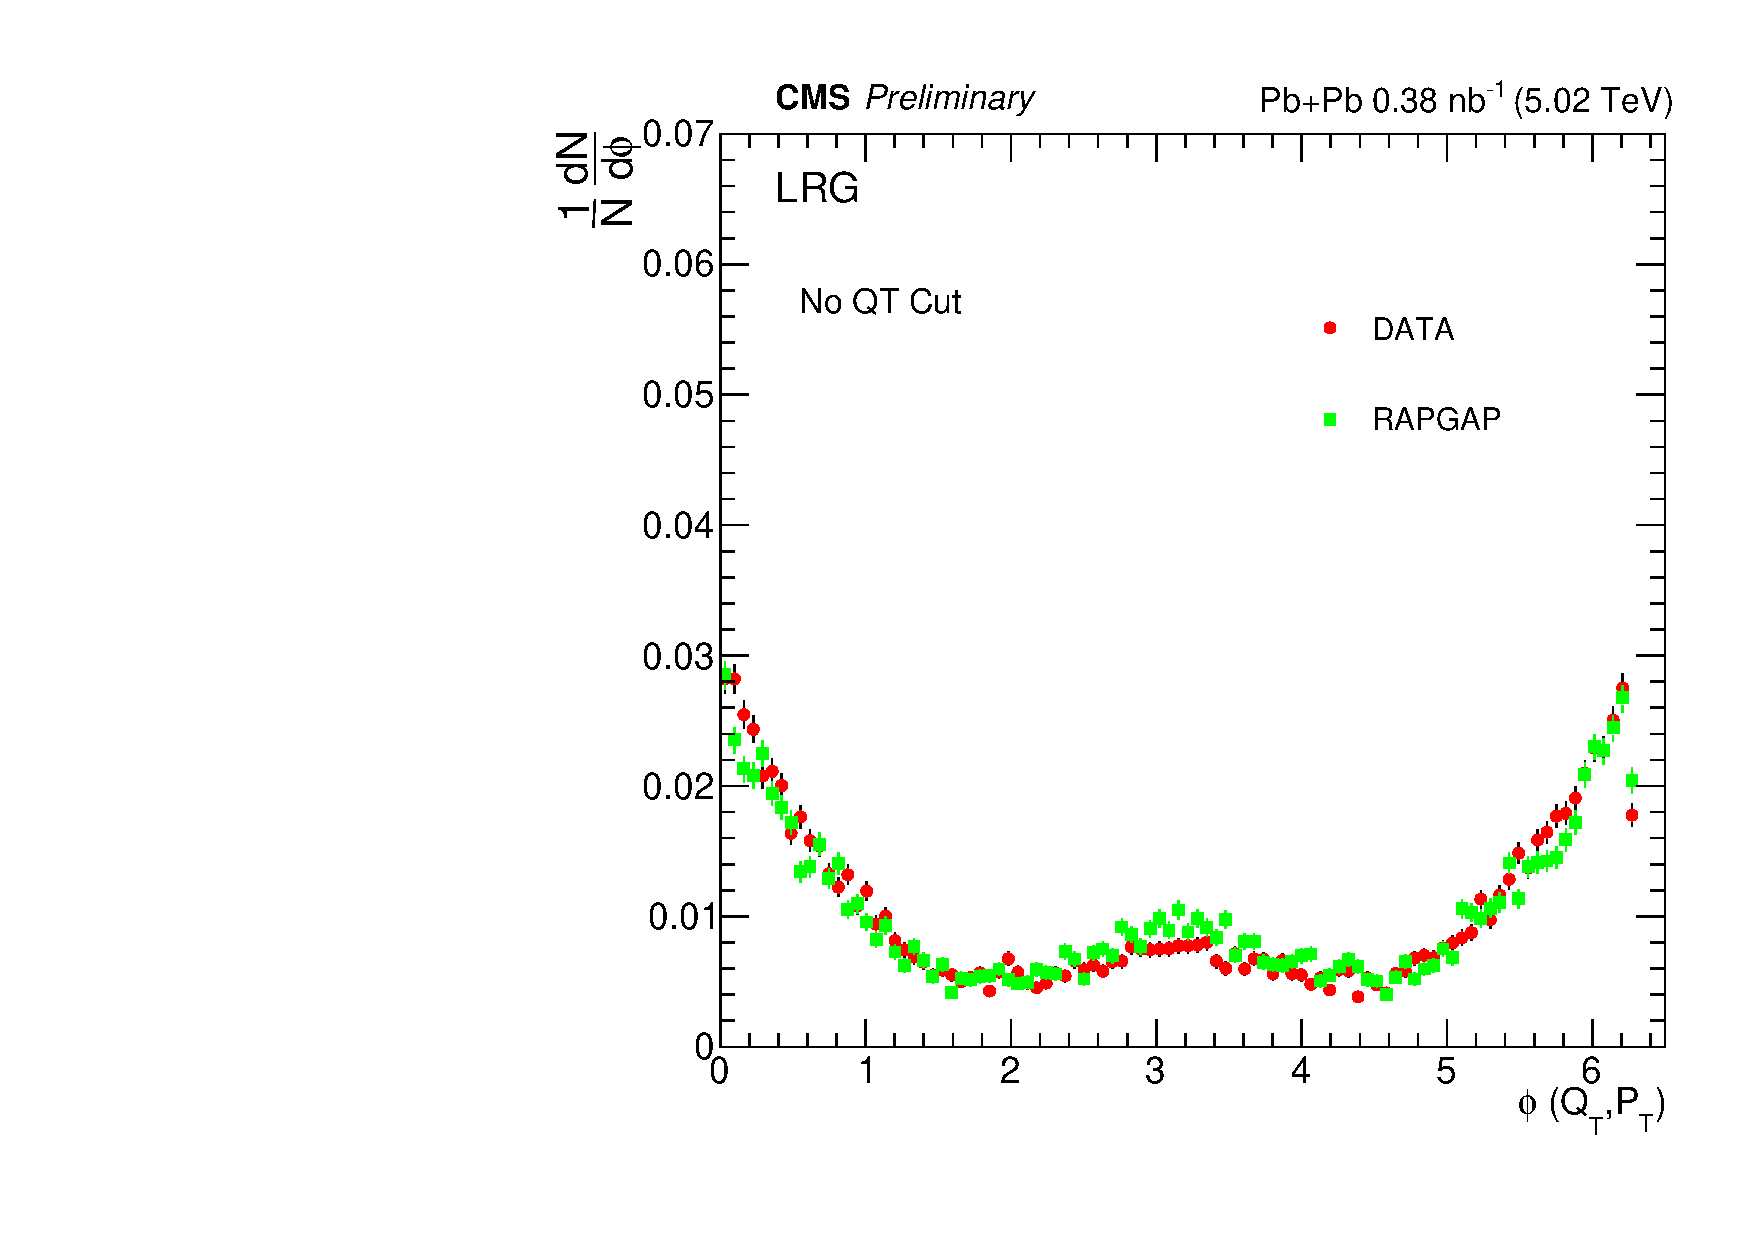
\includegraphics[width=6in]{Chapter6/importfigs/phi_allQt_raw.pdf}
\par\end{centering}
\caption{Raw $\phi$ distribution. \label{fig:rawPhi}}
\end{figure}

The event-mixing method was used to account for the acceptance effects within CMS. The dijets of two separate events are mixed to assure that any correlations are not the result of physics. The distribution of mixed-data and mixed-gen MC is shown in figure \ref{fig:mixPhi}.

\begin{figure}[h!]
\begin{centering}
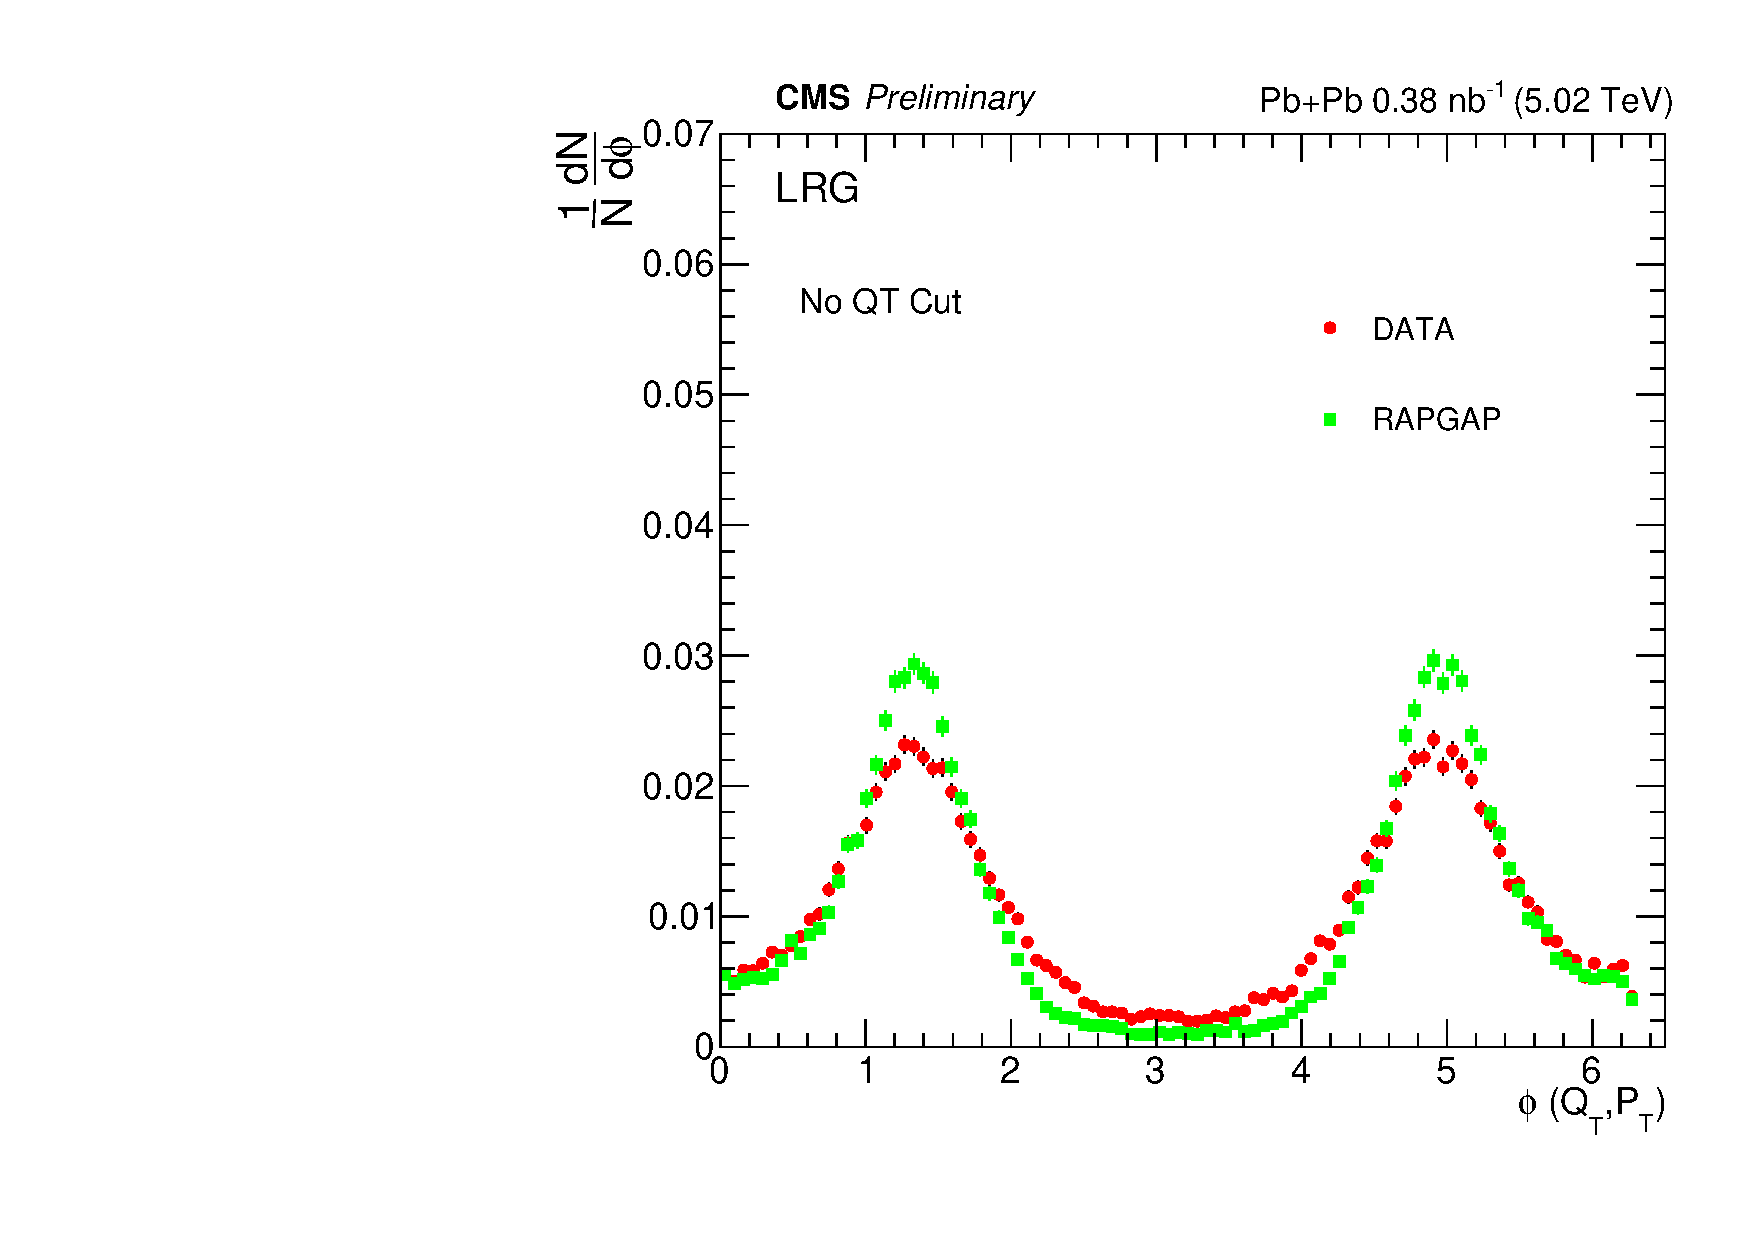
\includegraphics[width=6in]{Chapter6/importfigs/phi_allQt_mixed.pdf}
\par\end{centering}
\caption{Mixed $\phi$ distribution. \label{fig:mixPhi}}
\end{figure}

The "mixed" $\phi$ distribution is subtracted from the "raw" $\phi$ distribution. The "subtracted" $\phi$ distributions are shown in figure \ref{fig:subPhi}.

\begin{figure}[h!]
\begin{centering}
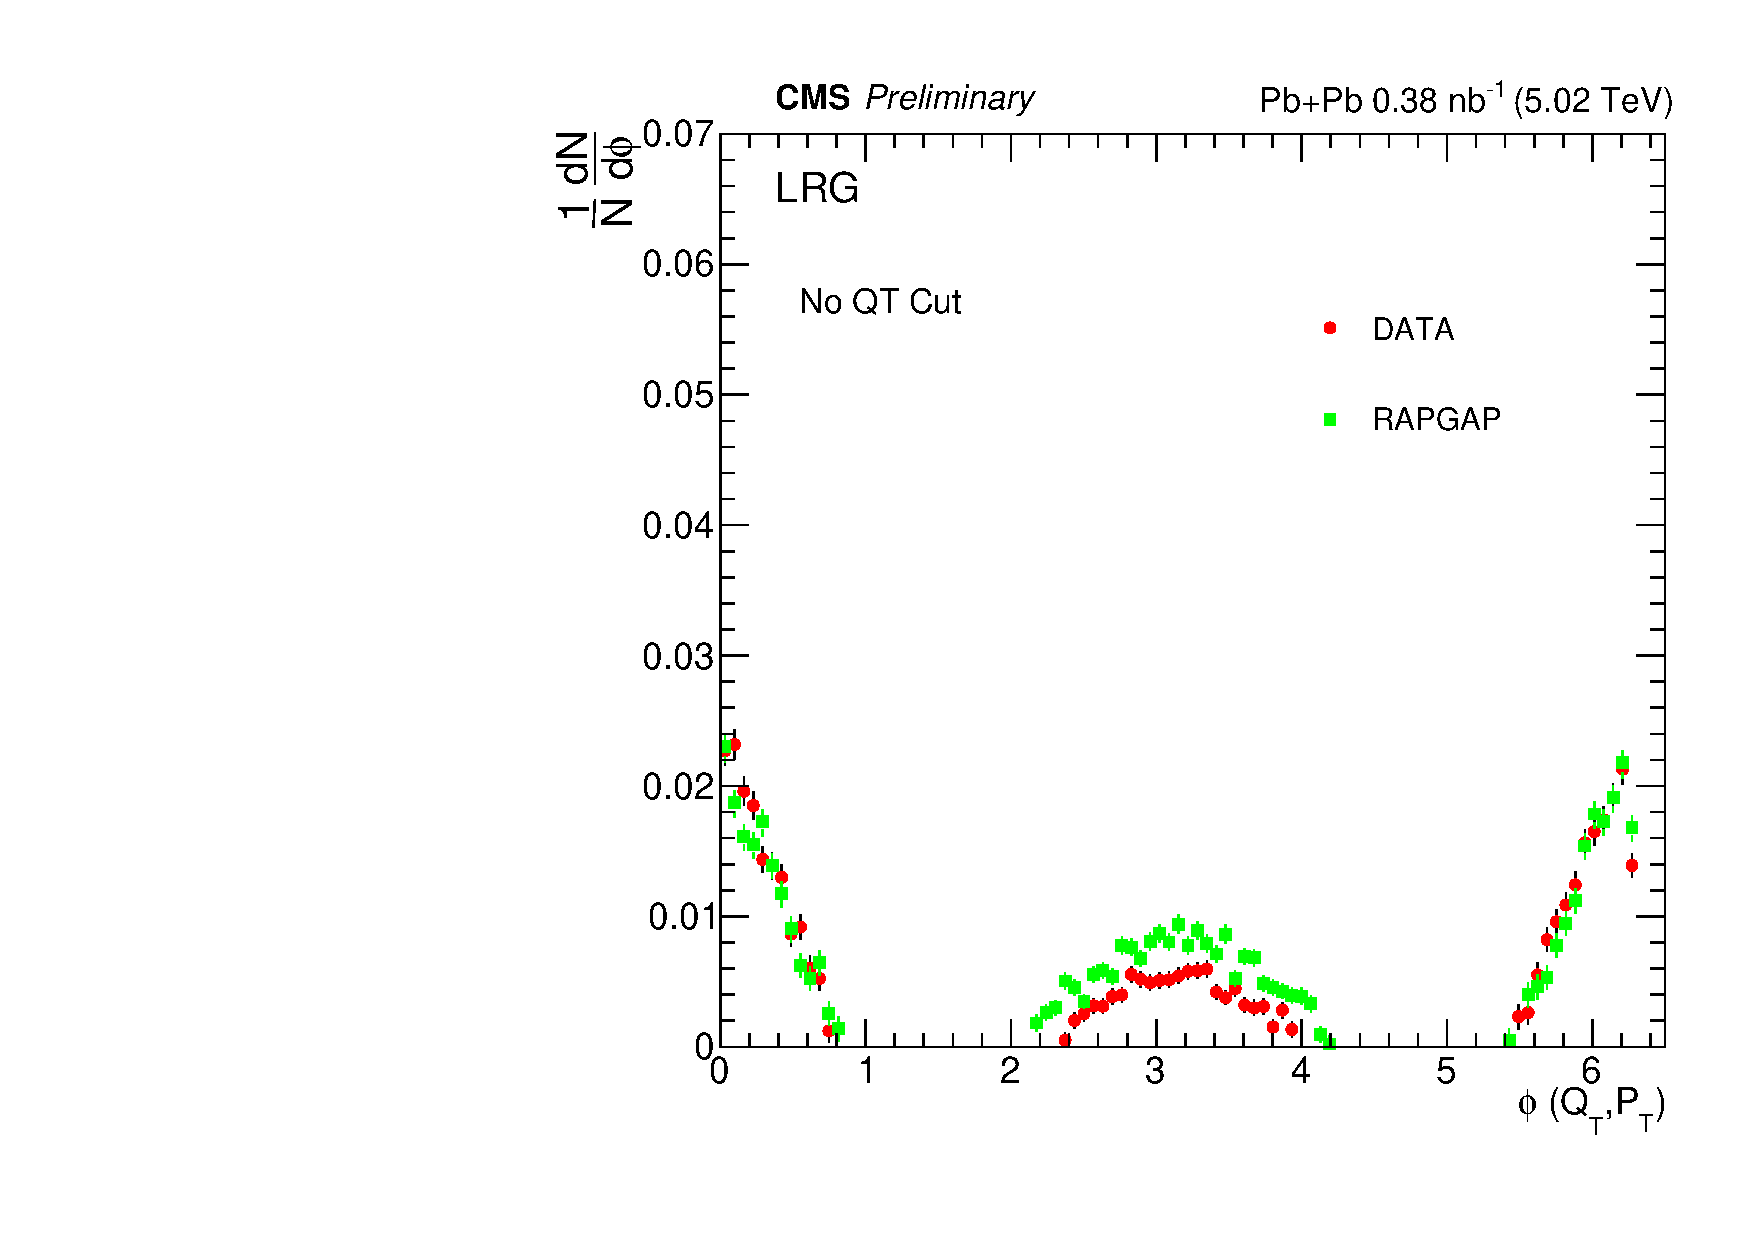
\includegraphics[width=6in]{Chapter6/importfigs/phi_allQt_subbed.pdf}
\par\end{centering}
\caption{Subtracted $\phi$ distribution. \label{fig:subPhi}}
\end{figure}

There is an additional R-factor that must be applied to account for the resolution of CMS. The corrected $\phi$ distribution can be seen in figure \ref{fig:finPhi}. 

\begin{figure}[h!]
\begin{centering}
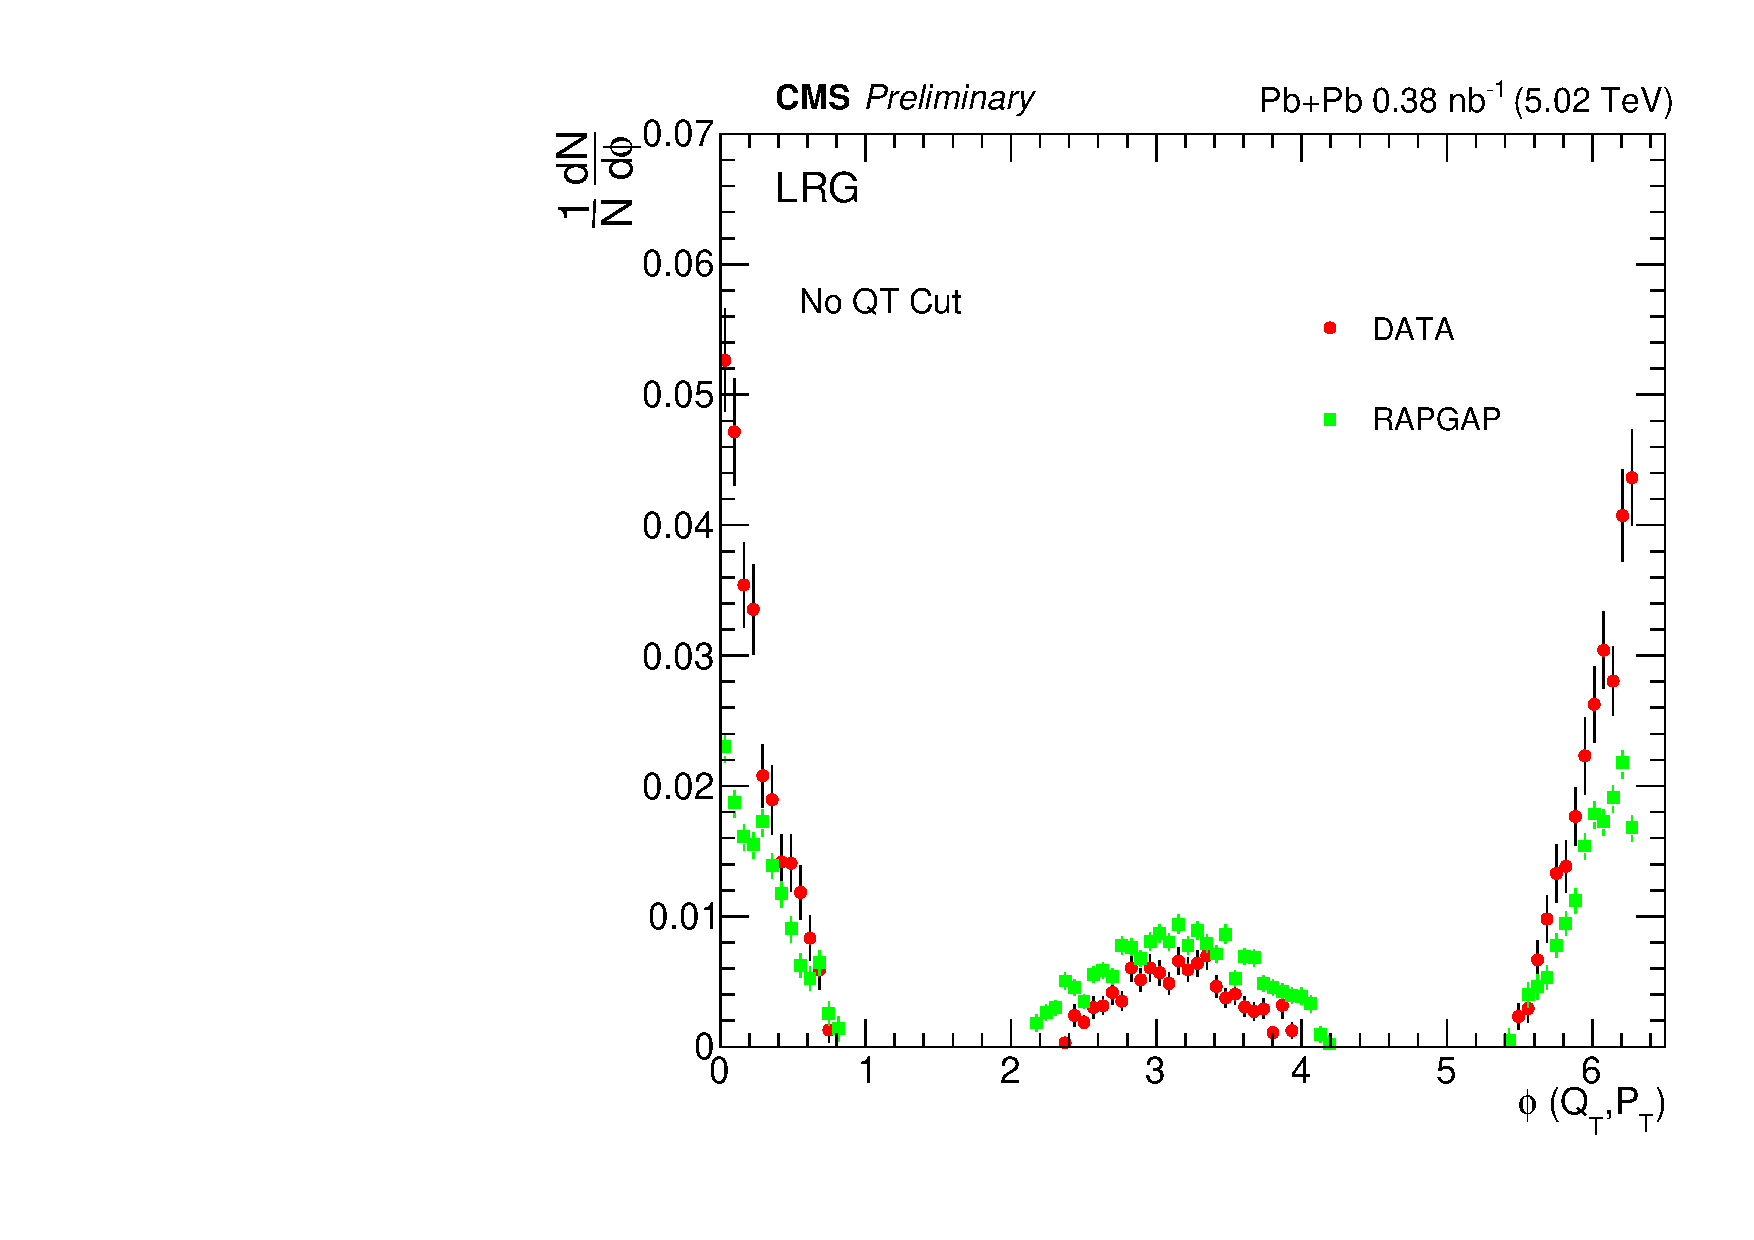
\includegraphics[width=6in]{Chapter6/importfigs/phi_allQt_final.pdf}
\par\end{centering}
\caption{Final $\phi$ distribution. \label{fig:finPhi}}
\end{figure}